\documentclass[a4paper,11pt]{article}
\usepackage[left=2.5cm, right=2.5cm, top=1.5cm, bottom=1.5cm]{geometry}
\usepackage{graphicx}
\usepackage{amssymb}
\usepackage{amsmath}
\usepackage[procnames]{listings}
\usepackage{xcolor}
\usepackage[numbered]{mcode}
\usepackage{hyperref}

\hypersetup{ %color attributes of citation, link, etc.
    colorlinks=true,
    linkcolor=blue,
    filecolor=gray,
    urlcolor=blue,
    citecolor=blue,
}

\setlength{\parindent}{0pt}


\newcommand{\matlab}{\textsc{Matlab}} %very important and totally necessary addition
\newcommand{\parallelsum}{\mathbin{\!/\mkern-5mu/\!}}

\newcommand\Item[1][]{%
  \ifx\relax#1\relax  \item \else \item[#1] \fi
  \abovedisplayskip=0pt\abovedisplayshortskip=0pt~\vspace*{-\baselineskip}}

%'codify' text for snippets
\definecolor{codegray}{gray}{1}
\newcommand{\code}[1]{\colorbox{codegray}{\texttt{#1}}}
           
\begin{document}
\title{\LARGE{\textbf{ECEN425 Mechanical Principles Assignment}}}
\author{Niels Clayton : 300437590}
\date{}
\maketitle
\hrule

\begin{enumerate}
   
    \item 
    $ \mathrm{Loss \; of \; function \; parameter} = \pm10\% $ \\
    $\mathrm{Maximum \; allowable \; parameter} = \pm30\%$\\
    Nominal Failure = $500N$

    \begin{align*}
        n_d&=\frac{\mathrm{loss \; of \; function \; parameter}}{\mathrm{maximum \; allowable \; parameter}}\\
        &= \frac{1/0.9}{1/1.3} \\
        &= 1.444\\\\
        \mathrm{Max. \; allowable \; load} &= \frac{500}{1.444} \\
        &= 346.26N
    \end{align*}

    \item 
    $n_d = 2.0$ \\
    Nominal Failure = $100N$
    
    \begin{align*}
        \mathrm{Max. \; allowable \; load} &= \frac{\mathrm{loss \; of \; function \; parameter}}{n_d}\\
        &= \frac{100}{2.0} \\
        &= 50N
    \end{align*}

    \item 
    $P = 8896N$\\
    $S = 165.5MPa$\\
    $n_d = 3.0$        

    \begin{align*}
        n_d&=\frac{\mathrm{loss \; of \; function \; stress}}{\mathrm{maximum \; allowable \; stress}} = \frac{S}{\sigma}\\
        \sigma &= \frac{165.5MPa}{3.0}\\
        &= 55.1\bar{6}MPa\\\\
        A &= \frac{P}{\sigma}\\
        &= \frac{8896N}{55.1\bar{6}MPa}\\
        &= 161.26mm^2\\\\
        d&= 2\sqrt{\frac{A}{\pi}}\\
        &= 14.33mm
    \end{align*}

    \item 
    $P = 100N$\\
    $r = 5mm$

    \begin{align*}
        \sigma &= \frac{P}{A}\\
        &= \frac{P}{\pi r^2}\\
        &= \frac{100}{25\pi}\\
        &= 1.27MPa\\
    \end{align*}

    \item 

    \subsection*{Matlab used for plotting}
    \lstinputlisting{Assignment4.m}
    \vspace{15pt}
    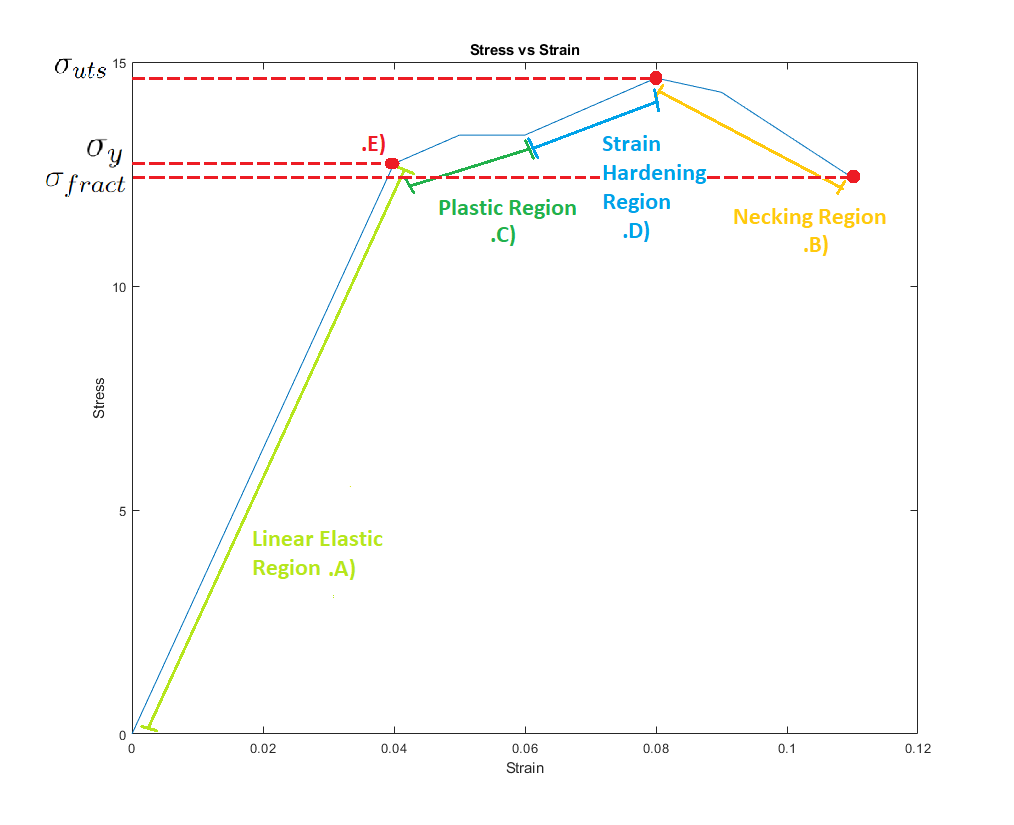
\includegraphics[width= \textwidth ]{q5.png}


    \item 

    \begin{enumerate}
        \item 

        \begin{align*}
            E &= \frac{\Delta\sigma}{\Delta\epsilon}\\\\
            &= \frac{12.7324}{0.04}\\
            &= 0.318GPa
        \end{align*}

        \item 
        Plastics such as HDPE (High Density Poly Ethylene) have a Young's modulus of approximately 0.8GPa, while metals like steel have a Young's modulus of approximately 100GPa. This suggests that this material is a thermoplastic rather than a metal. 

        \item 
        Our stress strain diagram assumes that the diameter of the sample being tested remains constant. This results in the flat and descending slopes that we see on our plot. This is due to the sample deforming and the diameter decreasing.\\

    \end{enumerate}

    \item 
    $\sigma_y = 500Mpa$\\
    $\epsilon_y = 0.02$

    \begin{align*}
        U_r&=\frac{\sigma_y \epsilon_y}{2}\\
        &= \frac{500 \times 0.02}{2}\\
        &= 5Nmm^{-2}
    \end{align*} 
    
    \item 

    \begin{enumerate}
        \item 
        $P = 3000kg$f\\
        $D = 10mm$\\
        $d = 5mm$\\

        \begin{align*}
            BHN &= \frac{2P}{\pi D \left[ D - \sqrt{D^2 - d^2} \right]}\\\\
            &= \frac{2 \times 3000}{10\pi \left[ 10 - \sqrt{100 - 25} \right]}\\\\
            &=142.55
        \end{align*}
        
        \item The Brinell hardness test provides a better approximation of the average hardness then the Rockwell hardness test. This is due to the much larger indenter used in the test.

    \end{enumerate}

    \item 

    \begin{enumerate}
        \item No, a clean fracture means there is little to no plastic deformation, making the brittle.

        \item No, a brittle material is likely to fracture and break under collisions with ice-sheets. An icebreaker boat make from this material would be redundant, as it would probably sink due to the collision of the wine bottle at its christening.  
    \end{enumerate}

    \newpage

    \item 
    $d_0 = 14.0mm$\\
    $E = 111.0GPa$\\
    $\nu = 0.349$\\
    $P = 20kN$

    \begin{align*}
        \sigma &= \frac{P}{A} = \frac{P}{\pi r^2} = \frac{20}{49 \pi }\\
        &= 0.13 GPa\\\\
        \epsilon_{long} &= \frac{\sigma}{E} = \frac{0.13GPa}{111.0GPa}\\
        &= 1.17\times10^{-3}\\\\
        \epsilon_{lat} &= -\nu \times \epsilon_{long} = 0.349 \times 1.17\times10^{-3}\\
        &= -4.08\times10^{-4}\\\\
        \Delta d &=  \epsilon_{lat} \times d_0 \\
        &= -5.72\times10^{-3}\\\\
        d_f &= d_0 + \Delta d\\
        &= 13.9942mm
    \end{align*}

    \item 
    $l_0 = 100mm$ , $l_f = 100.559$\\
    $d_0 = 10mm$, $d_f = 9.980mm$\\
    $P = 50N$\\
    $E = 114.0GPa$\\

    \begin{align*}
        \Delta d &=  d_f - d_0 = 9.980 - 10\\
        &= -0.02\\\\
        \epsilon_{lat} &= \frac{\Delta d}{d_0} = \frac{-0.02}{10}\\
        &= -2 \times 10^{-3}\\\\
        \Delta l &=  l_f - l_0 = 100.559 - 100\\
        &= 0.559\\\\
        \epsilon_{long} &= \frac{\Delta l}{l_0} = \frac{0.559}{100}\\
        &= 5.59 \times 10^{-3}\\\\
        \nu &= -\frac{\epsilon_{lat}}{\epsilon_{long}} = -\frac{-2 \times 10^{-3}}{5.59 \times 10^{-3}}\\
        &= 0.357
    \end{align*}

    The calculated Poisson's is closest to that of Magnesium ($\nu = 0.350$). However it should be noted that this is also very close to phosphor bronze ($\nu = 0.349$). 

    \item 
    $P = 2kN$

    \begin{align*}
        \tau_{avg}&= \frac{V}{A} = \frac{2kN}{192mm^2}\\
        &= 10417kPa
    \end{align*}

    
    \item 
    $\tau = 500kPa$\\
    $n_d = 2.0$\\
    $V = 20kN$\\

    \begin{align*}
        \mathrm{Max. \; allowable \; load} &= \frac{\mathrm{loss \; of \; function \; parameter}}{n_d}\\
        &= \frac{\tau}{n_d}  = \frac{500kPa}{2.0}\\
        &= 0.00025GPa\\\\
        A &= \frac{V}{\tau} = \frac{20kN}{0.00025GPa}\\
        &= 80000mm^2
    \end{align*}


\end{enumerate}
\end{document}